% Niveau :      PCSI
% Discipline :  Méca

\begin{exercise}{Chaises volantes}{2}{Sup}
{Mécanique,Pendule,Pendule conique}{bermudez}

Voici la photographie d'un manège de chaises volantes.

\begin{figure}[H]
    \centering
    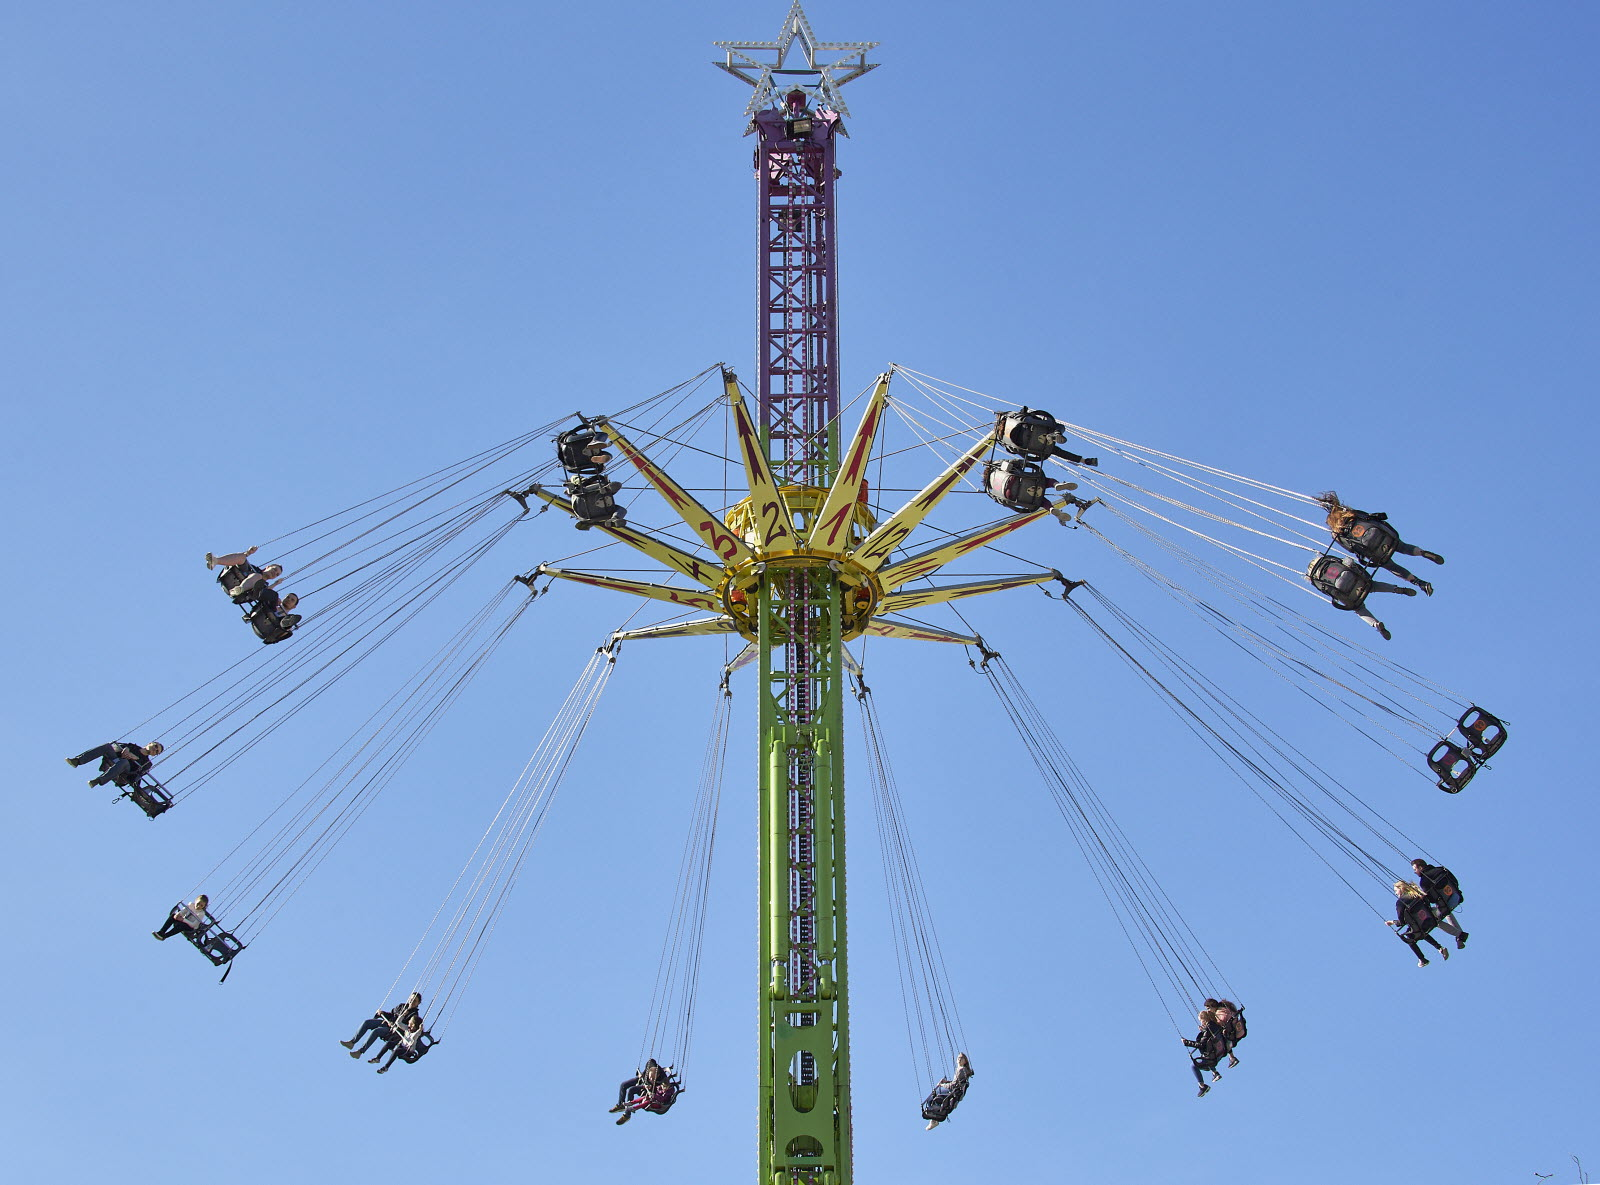
\includegraphics[width=\linewidth]{meca/mecapoint/chaises_volantes.png}
    \caption{Photographie du manège.}
    \label{fig:my_label}
\end{figure}

\textsf{Question ouverte :}~estimer la vitesse de rotation du manège, en rotations par minute.

\end{exercise}

\begin{solution}

Nous allons estimer la vitesse de rotation grâce à la dynamique d'une des chaises volantes, occupée par deux personnes.

Supposant qu'il s'agit d'une particule ponctuelle massive, dans le référentiel tournant, on connaît son accélération centripète due à la rotation $a = -R\Omega^2$. Celle-ci doit être compensée par la projection orthogonale de la force de tension des câbles, elle-même déterminée par la gravité ($g = \SI{9,81}{m^2\cdot s^{-1}}$) dans la direction verticale.

On estime grâce à la référence de taille connue, celle d'une personne assise, environ \SI{1}{m}, on peut estimer la longueur des câbles qui suspendent les chaises volantes : $L = \SI{10}{m}$, ainsi que l'angle entre la verticale et les câbles $\alpha = \SI{45}{deg}$.

On trouve donc :
$$\text{dans la direction $z$} : 0 = -mg + T\cos{\alpha}$$
$$\text{dans la direction $r$} : -mR\Omega^2 = -T\sin{\alpha}$$

Or connaissant également $R = L\sin\alpha$, on obtient :
$\Omega = \sqrt{\dfrac{g}{L\cos\alpha}}$

Ainsi sommes-toute : $\Omega = (\cos\alpha)^{-1/2} = \SI{1.2}{rad\cdot s^{-1}} = \SI{11}{rpm}$.

\end{solution}